\subsection{Ants’ Foraging Behavior in real life}
When finding the way, ants exchange information indirectly and operate in a self-organizing manner. Despite its simplicity, this method allows the ants to perform complex tasks that are far beyond the ability of individual ants, especially the one to find the shortest path from their nest to the food source, even though they are unable to measure path length. 
While moving, ants deposit a chemical called pheromone. Ants can smell the pheromone and they tend to choose paths marked by strong pheromone concentrations. Based on this trait, ants can follow the path to the food source discovered by other ants. Overall, This collective trail-laying and trail-following behavior whereby an ant is influenced by a chemical trail left by other ants is the inspiration of \gls{aco}~\cite{parsons2005ant}.

One of the most well-known experiments on ant's pheromone trail-laying and -following behavior is the Double bridge experiment, designed and conducted by Deneubourg~\textit{et al}. The experiment was simply set up with a double bridge placed between the ant nest and the food source (See Figure~\ref{fig:aco_exp}). Besides, the ratio $r = l_l / l_s$ between the length of the two branches of the double bridge is varied, where $l_l$ was the length of the longer branch and $l_s$ the length of the shorter one.

The first experiment is illustrated in Figure~\ref{fig:aco_exp_1}, where the bridge has two equal branches ($r = 1$). At the start, the ants randomly choose a path from the nest to the food source. Over time, all the ants used the same branch. This could be explained by the amount of pheromone spread out over time by the ants. First, the ant will randomly choose one of the two branches because there are no pheromones. Due to random fluctuations, the number of ants on each branch is not equal. A few more ants choose one branch over the other, which means a larger amount of pheromone is deposited in only one branch. This higher concentration of pheromone encourages other ants to pick that branch again, and so on until the ants all converge to one single path.

The second experiment was set up similarly to the first, however, $r = 2$, i.e. the long branch was twice as long as the short one (See Figure~\ref{fig:aco_exp_2}). In this case, the ants that choose the shorter branch will be the first to reach the food source and vice versa. Consequently, the shorter branch will concentrate a larger amount of pheromone, thus biasing the ant's decision in its favor. Therefore, after a while, nearly all the ants chose to use only the short branch. It is interesting to note that not all ants utilize the short branch, with just a tiny fraction opting for the longer one.

Figure~\ref{fig:aco_exp_3} demonstrated the final experiment. Initially, only one long branch was placed between the nest and the food source. After 30 minutes, a new short one is added. As a result, the short branch was picked sporadically and the colony was stuck on the long branch. The reason for this may due to the high pheromone concentration on the long branch and the slow evaporation rate of the pheromone. Because of its high pheromone concentration, the long branch is chosen by the majority of ants, which keeps reinforcing the long branch even when a shorter one arrives. At the same time, the evaporation rate of the pheromone is also too slow for the ants to forget the suboptimal path they have previously converged on so that a new path can hardly be discovered.

\setlength{\intextsep}{4pt}
\renewcommand{\scalefigure}{0.5}
\begin{figure}[htbp]
	\centering
	\begin{subfigure}{.49\linewidth}
		\centering
		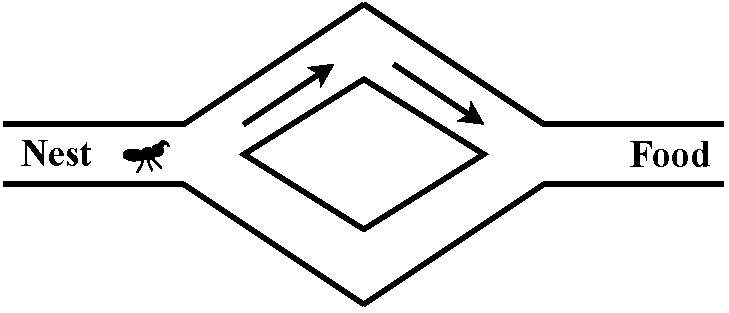
\includegraphics[scale=\scalefigure]{Figures/chap 1/Ant Experiment.pdf}
		\caption{Branches have equal length}
		\label{fig:aco_exp_1}
	\end{subfigure}
	\begin{subfigure}{.49\linewidth}
		\centering
		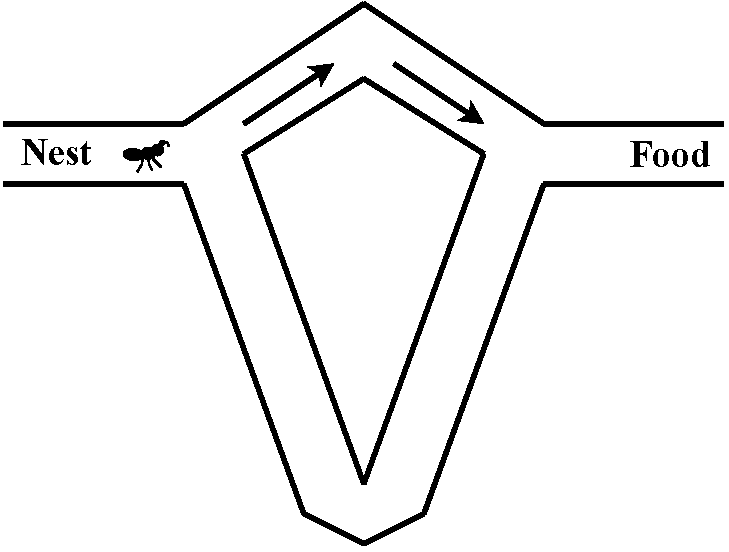
\includegraphics[scale=\scalefigure]{Figures/chap 1/Ant Experiment 2.pdf}
		\caption{Branches have different length}
		\label{fig:aco_exp_2}
	\end{subfigure}

	\begin{subfigure}{.95\linewidth}
		\centering
		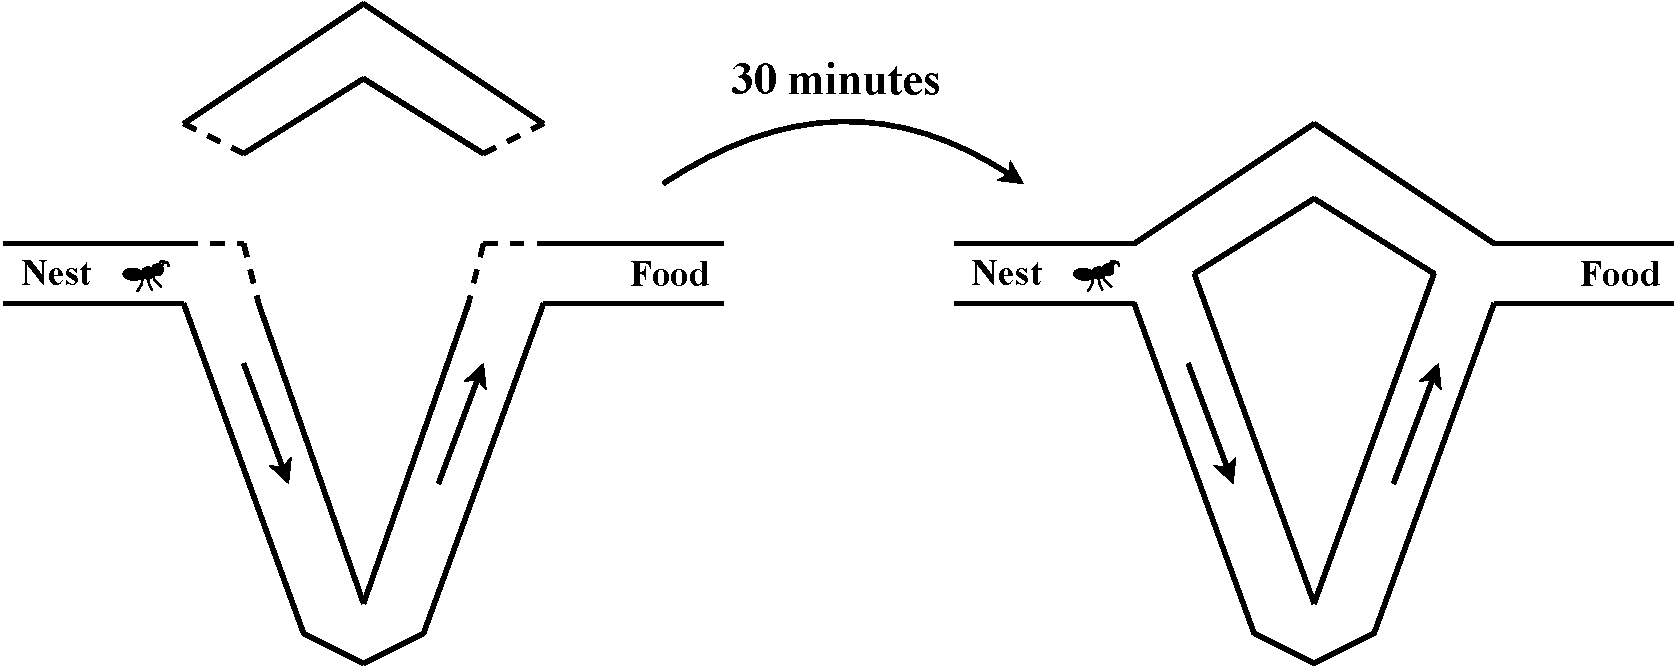
\includegraphics[scale=\scalefigure]{Figures/chap 1/Ant Experiment 3.pdf}
		\caption{Only the long branch was setup to the colony at first. After 30 minutes, a new shorter one is added.}
		\label{fig:aco_exp_3}
	\end{subfigure}
	\caption{Experimental setup for the Double bridge experiment.}
	\label{fig:aco_exp}
\end{figure}

\subsection{General Ant Colony Optimization - Ant System}
\acrfull{aco}, which is a population-based metaheuristic and suitable for solving discrete optimization problems, was first proposed by Dorigo~\textit{et al.}~\cite{dorigo1996ant} in the year 1996. Unlike natural ants, as an optimization tool, each of the artificial ants in the \gls{aco} is equipped with exceptional features. Ant chooses its path based on probability, which is proportional to the pheromone concentration and inversely proportional to the path's cost. To avoiding roaming, the ant saves its journey in the memory. When it reaches the destination, the ant updates a corresponding quantity of pheromone on each traversed path. Algorithm~\ref{alg:as} outlines the skeleton of the \gls{as} algorithm, which is the first one pertaining to \gls{aco} classes proposed.
\bigskip
\begin{algorithm}
	\caption{The pseudocode of \gls{as}}
	\label{alg:as}
	\Begin
	{	
		Initialize \tcp*{Initialize the pheromone matrix and $m$ ants}
		\While{terminate conditions are not satisfied} 
		{
			Place each ant in a starting node\;
			\While{all ants have not finish building their solutions} 
			{
				\ForEach{ant}
				{
					Choose next node by applying~\ref{eq:aco_transition} \;
					Update trail\;
				}
			}
		}
	}
\end{algorithm}
\bigskip
Initially, the trail intensity on all routes was initialized equal and regularly with a small value. Subsequently, the algorithm iterates itself until it accomplishes the termination criteria. This process consists of the following sequential stages: In the first stage, the ants start from their nest and find their way. To travel from node $i$ to $j$, the $k^{th}$ ant must choose an edge in the $available_k$ through a transition probability function:
\begin{equation}
\label{eq:aco_transition}
p^k_{ij} =
\begin{cases}
	\frac{[\tau_{ij}(t)]^{\alpha} \cdot [\eta_{ij}(t)]^{\beta}} {\Sigma_{k \in available_k} [\tau_{ik}(t)]^{\alpha}\cdot [\eta_{ik}(t)]^{\beta}}, & \text{if $j \in available_k$}, \\
	0, & \text{otherwise}
\end{cases}
\end{equation}
where $\eta_{ij}$, which is equal to $1/d_{ij}$, defines the "attractive" of edge $(i,j)$ to the ant. $\alpha$ and $\beta$ are two parameters that play roles in control the relative importance of the pheromone trail versus the ant's experience. Apparently, the route selection is a trade-off between routes that were most previously visited by the other ants in the colony or implementing an empirical greedy heuristic. 

Whenever all ants have ended their journey at the destination, the pheromone trail $\tau_{ij}$ at time $t+n$ is updated based on the evaporation rate $\rho$ and the added pheromone of ants $\Delta \tau_{ij}$.  
\begin{equation}
	\label{eq:aco_update}
	\tau_{ij}(t+n) = \rho \cdot \tau_{ij}(t) + \Delta \tau_{ij}
\end{equation}
\begin{equation}
	\label{equa:aco_add}
	\Delta \tau_{ij} = \Sigma^m_{k=1} \Delta \tau_{ij}^k
\end{equation}
\begin{equation}
	\label{equa:aco_pher}
	\Delta \tau_{ij}^k = 
	\begin{cases}
		\frac{Q}{L_k} , & \text{if $k^{th}$ ant uses edge $(i,j)$ in its tour},\\
		0, & \text{otherwise},
	\end{cases}  
\end{equation}
where $\Delta \tau_{ij}^k$ is the amount of pheromone substance per unit of length laid on edge $e$ by the $k^{th}$ ant between time $t$ and $t + n$, with $Q$ is a constant number, and $L_k$ is the tour length of the $k^{th}$ ant.

The best solution is updated if the ant colony finds a better one. \gls{aco} finally returns the best solution when the stop condition is met.

%\subsection{Some variants of Ant Colony Optimization}
%\subsubsection{Ant Colony System}

%\subsubsection{Max-min Ant System}
